\section{Part B}

This second part of the problem aims to implement the pressure-velocity coupling and show how an arbitrary velocity field, after substracting the gradient of a certain type of field, can become a null-divergence one.

\subsection{Algorithm}

The implemented algorithm follows a simplified version of a predictor-corrector scheme. The objective is to begin with a velocity field containing artificial divergence and apply a correction using a scalar field (pseudo-pressure) whose gradient will subtract the divergence component from the velocity.

\begin{enumerate}
    \item Create coordinate positions, initialize null velocity field and introduce artificial divergence at a specific grid point by setting its horizontal and vertical velocities to non-zero values.
    \item Compute the divergence of the predictor velocity field using a custom function.
    \item Construct Laplacian matrix for pressure Poisson equation, solve a linear system for pseudo-pressure using the Laplacian equation and the divergence field in vector form.
    \item Convert the pseudo-P vector back to 2D field format, then compute its gradients. Correct the velocity field using the calculated pseudo-P gradients. Then, compute the divergence of this new velocity field.
    \item Compare maximum values of divergence before and after correction.
    \item Plot the results.
\end{enumerate}

A relevant remark about this code are that the divergence and gradient are calculated in the physical domain excluding the halo, which is calculated after. Both divergence and gradient are calculated using finite difference approximation, forward difference in the case of the gradient and backward for the divergence, ensuring consistency with the staggered-grid scheme.

\subsection{Validation strategy}

The validation of the pressure-velocity coupling is based on a two-step comparison of the divergence field. First, the divergence of the artificially perturbed velocity field is computed and its maximum absolute value is recorded. This provides a quantitative measure of how far the initial field is from being divergence-free. The maximum absolute divergence is again measured after correcting the velocity field.

A successful implementation should yield a corrected velocity field whose divergence is close to zero everywhere. Specifically, the maximum divergence should drop by several orders of magnitude, confirming that the projection step has effectively enforced incompressibility.

\subsection{Results}

\begin{figure}[H]
    \centering
    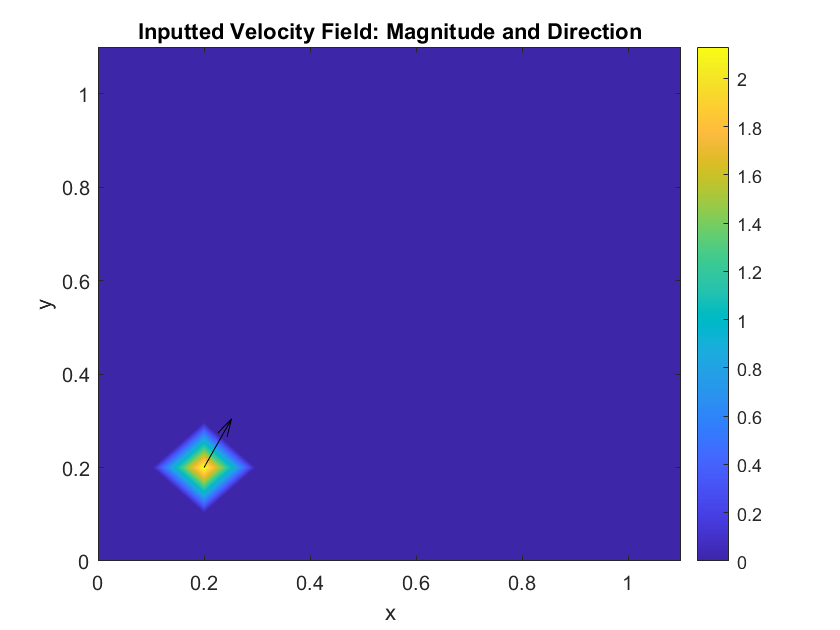
\includegraphics[width=0.7\linewidth]{imatges/InputV.png}
    \caption{Input non-zero velocity shown in the physical domain.}
    \label{fig:InputV}
\end{figure}

The visualization is consistent with with the injection of velocity in the null-velocity field.

\begin{figure}[H]
    \centering
    \includegraphics[width=0.7\linewidth]{imatges/PseudoP.png}
    \caption{Pseudo-pressure in the physical domain.}
    \label{fig:PseudoP}
\end{figure}

The pressure gradient is actively correcting the divergence introduced by the velocity. The gradient vectors align with regions of high pseudo-P variation.
